\chapter{Results}
In this chapter we will look at the performance of the fully tuned system in different simulation scenarios. Firstly we will look at how the temperature performs when starting at a stable state, then we move on to scenarios where we do different changes in the setpoint of the controller before we finish by looking at how the system behaves when doing a cold start.

\section{Stable startup}
When loading the conditions where the initial temperatures are about \SI{0.3}{\degreeCelsius} below deisred set point we get the response shown in \autoref{fig:stable_both}. Here we see that both the temperatures settles towards desired temperature within reasonable time, without any significant oscillations, and continues to work around this setpoint without large deviations due to noise. The controllers are also operating in an area where they are far from saturating, which is desirable. 

\begin{figure}[ht!]
	\centering
	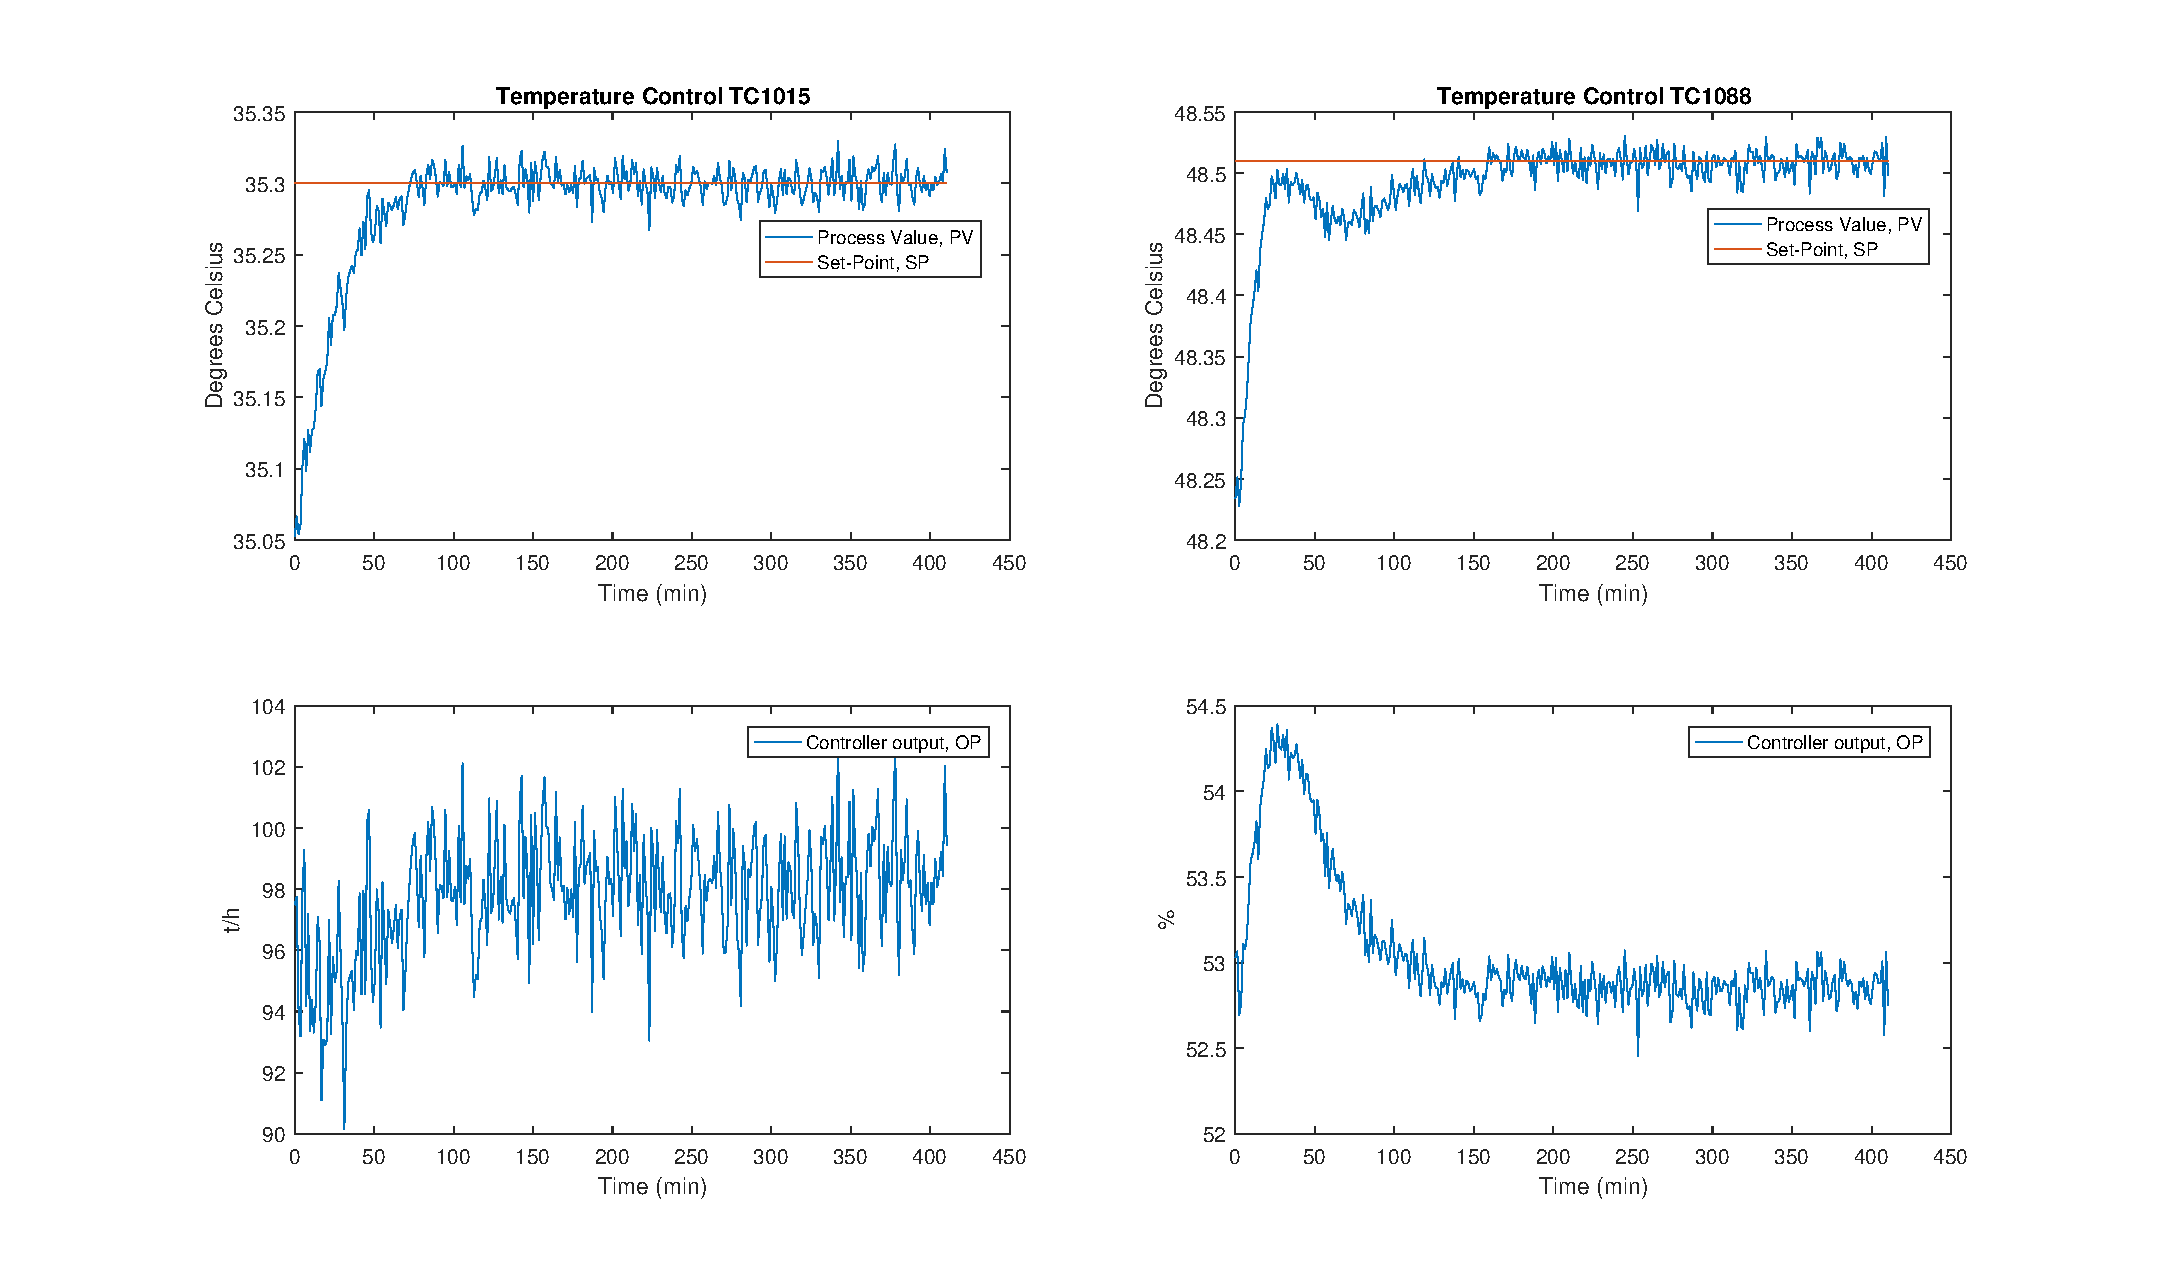
\includegraphics[width=0.95\textwidth]{fig/results/stable_both.eps}
	\caption{Response of both temperature controllers with initial conditions not at set point}
	\label{fig:stable_both}
\end{figure}

\clearpage
\section{Cold start}
When doing a cold startup, the process values are far off the desired checkpoints. This applies to both the temperature and level controllers. To reach the desired checkpoint we therefore need a lot of time. At a 15 hour simulation we see that we reach desired temperature in the top column fairly fast, while the response in the bottom column is slower. This is due to physical limitations in the system, as we see that the controller output from \texttt{24\_TC1088} are saturated at minimum. This output is the reference value for the controller \texttt{24\_LC1028} which controls the heat exhange area for the boilup part. As this is saturated as shown in \autoref{fig:lc1028_saturated} we see that there are no more room for more heat exchange, and this is a limitation for the system. It will take som time for the full plant to be in running condition after a cold start, as we need to wait for the temperature in the bottom column to reach its set point.

\begin{figure}[ht!]
	\centering
	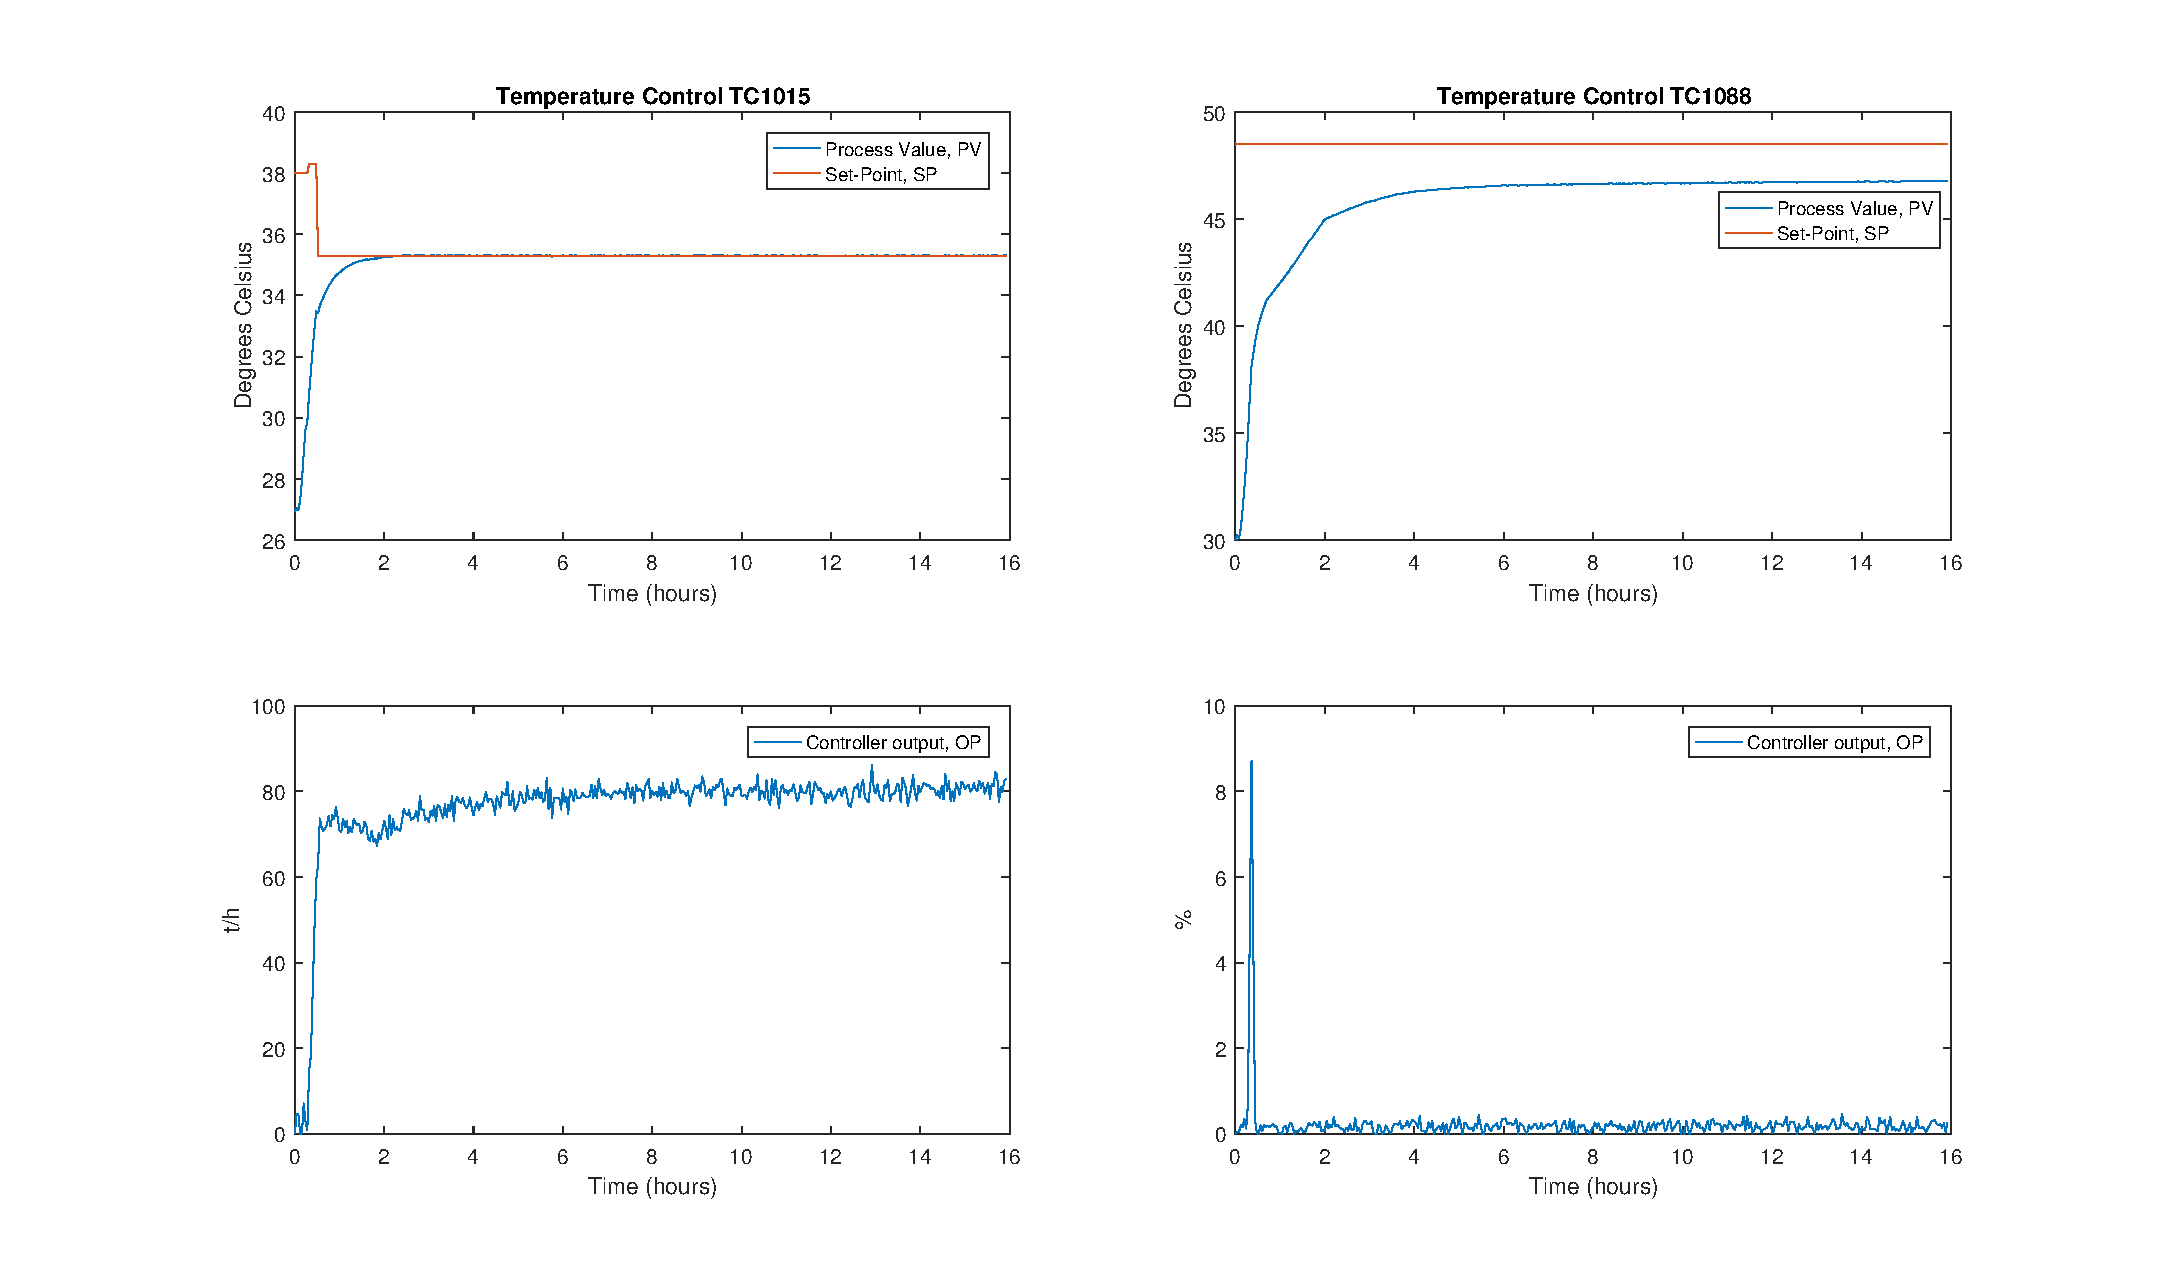
\includegraphics[width=0.95\textwidth]{fig/results/coldstart_both.eps}
	\caption{Output of both temperature controllers when doing a cold start of the system}
	\label{fig:coldstart_both}
\end{figure}

\begin{figure}[ht!]
	\centering
	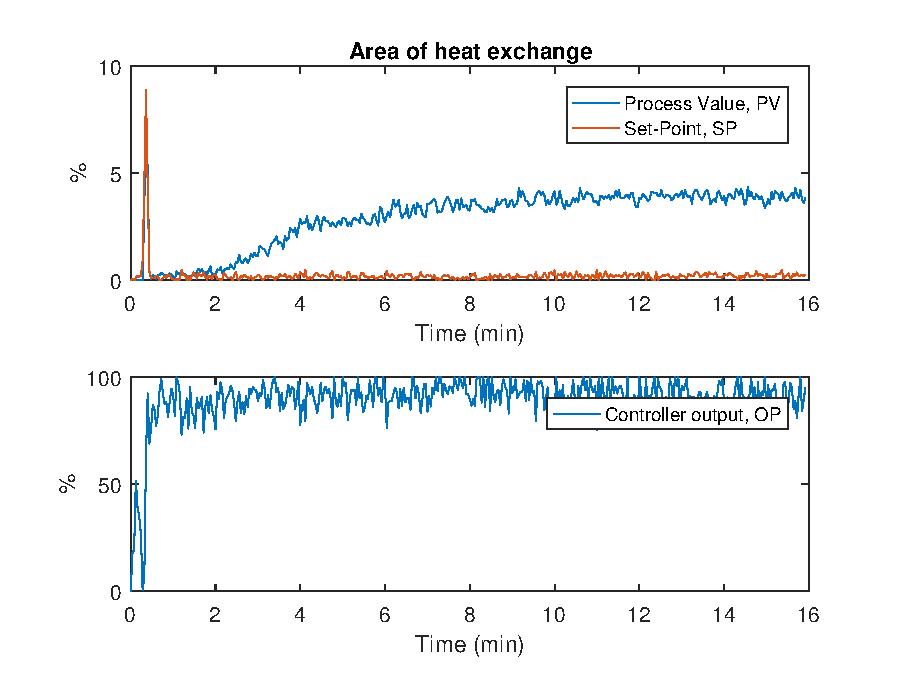
\includegraphics[width=0.95\textwidth]{fig/results/lc1028_saturated.eps}
	\caption{Controller for the heat exhange in the boilup part of the bottom column in saturation}
	\label{fig:lc1028_saturated}
\end{figure}

\clearpage
\section{Rapid step changes}
We now move on to a 12 hour simulation doing four step changes of $\pm$\SI{0.3}{\degreeCelsius}, two on each controller, we get the output shown in \autoref{fig:12h_steps}. Here wee see that both controllers follow reference good, although we see that when doing a change in the top column, this affects the bottom column quite alot more than the opposite direction. This is probably due to the fact that $K_p$ for \texttt{24\_TC1015} is severely larger than for \texttt{24\_TC1088} which again leads to more agressive tuning, which also can be seen in \autoref{fig:12h_steps}. Although this interaction we observe that both process values stays well within the specifications and there are no noticeable oscillations for this simulation. When looking at the time frame of this simulation, it's also fair to mention that we do many changes within a short time period and that the response with this set of controller parameters performs pretty decent.

\begin{figure}[ht!]
	\centering
	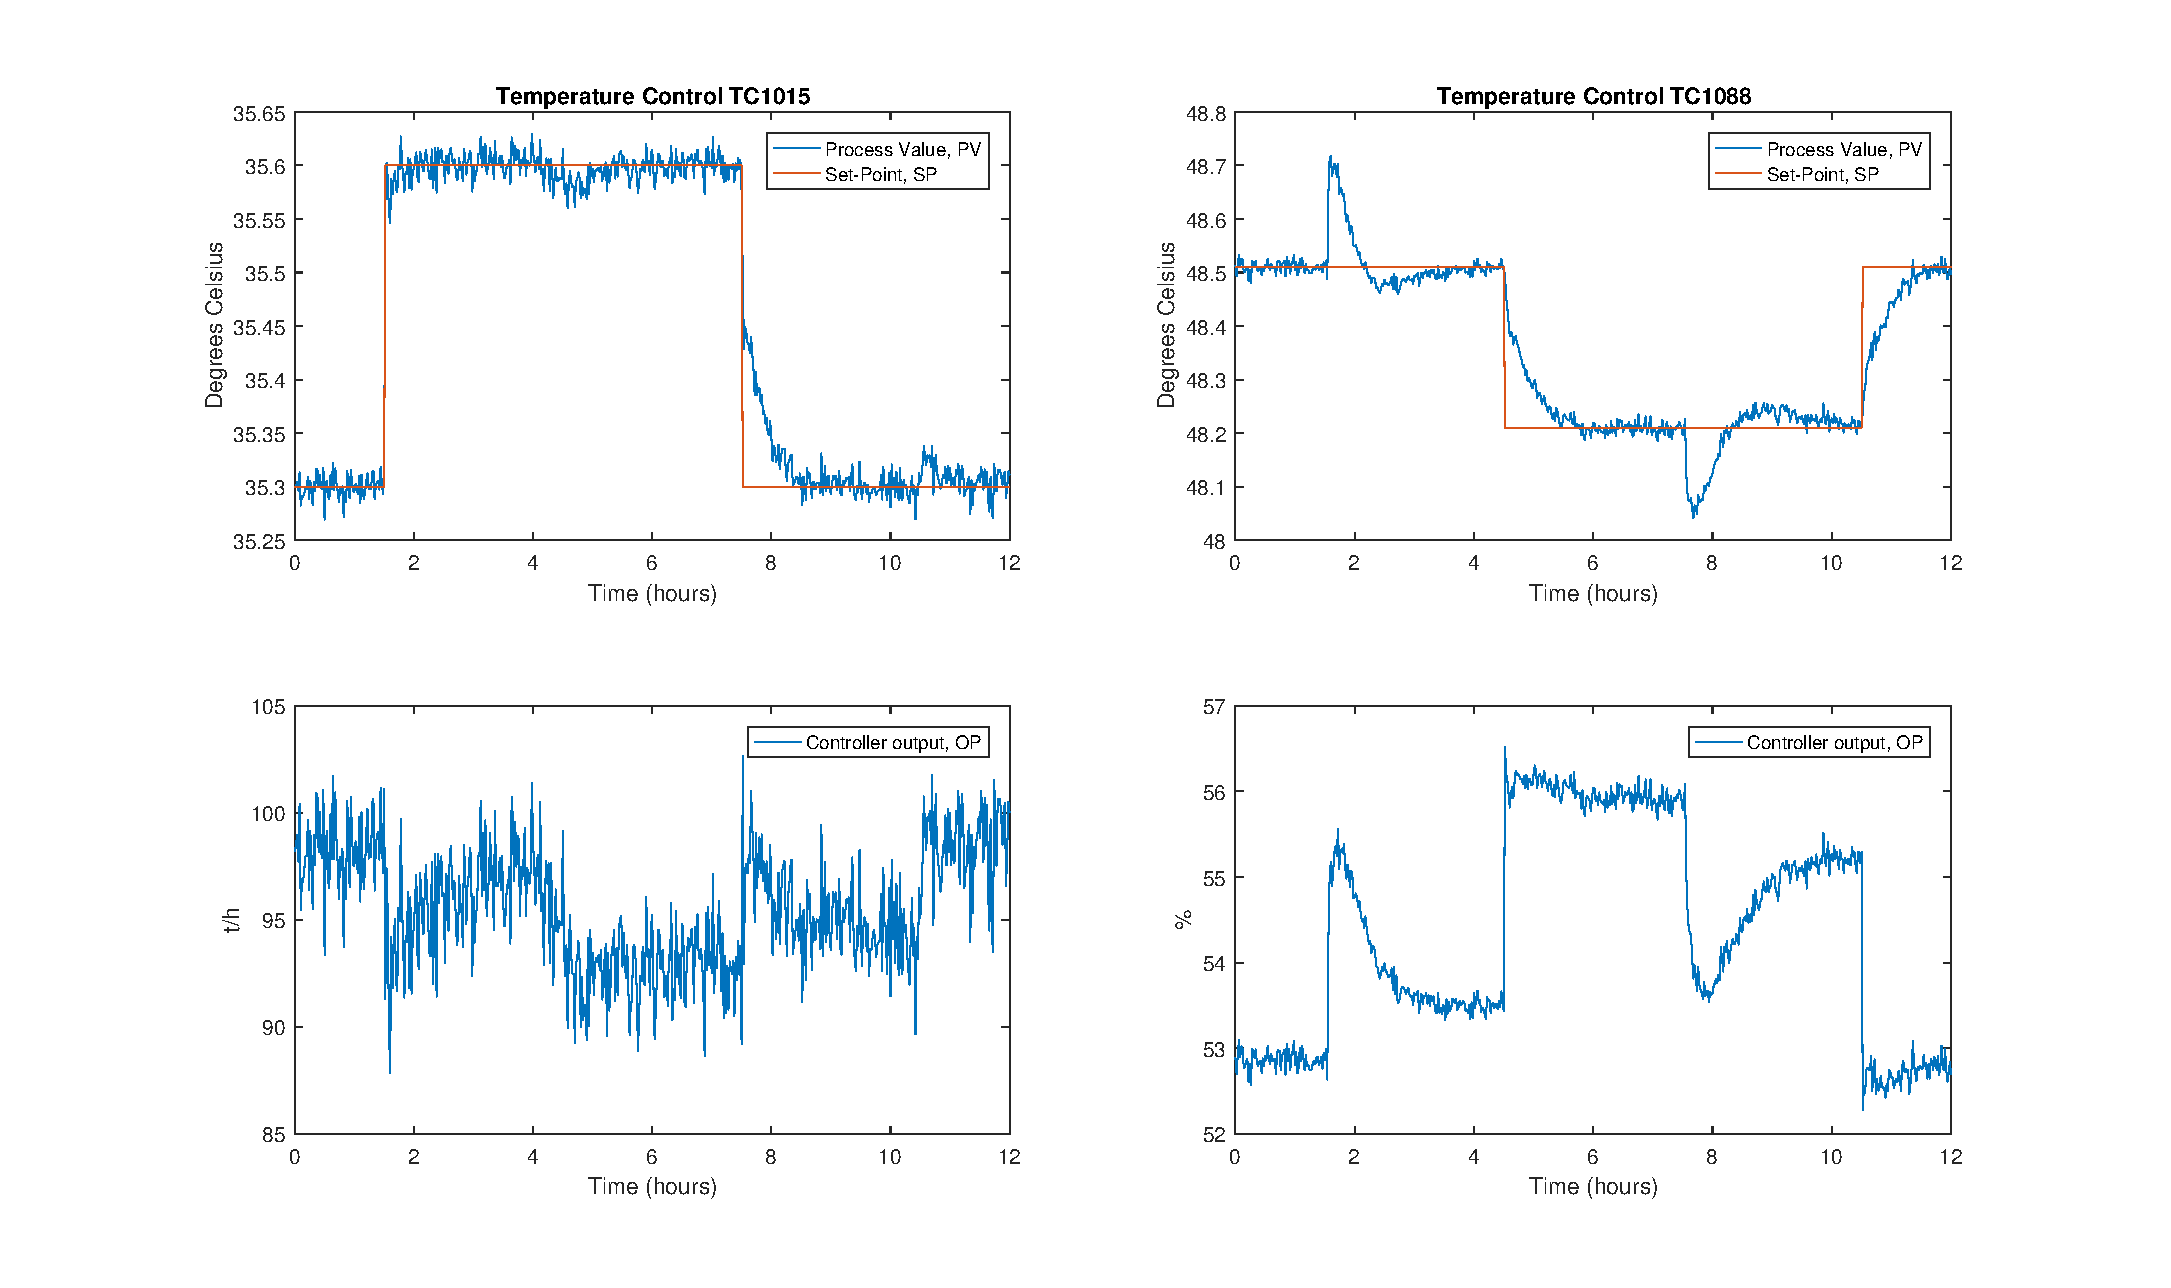
\includegraphics[width=0.95\textwidth]{fig/results/12h_steps_best.eps}
	\caption{Output of both temperature controllers when doing several steps within short time}
	\label{fig:12h_steps}
\end{figure}

\clearpage
\section{Summary}
All in all the plant now performs reasonably within the specifications and the controllers perform well by them selves. The controller parameters for the two temperature controllers could perhaps have been chosen slightly different to counteract the interations between the system, but as the system performs at this point, the paramaeters will be kept as is, as the controllers works their way back from these deviations within reasonable time. When it comes to the cold start up, we saw that the time until the system is properly running is long due to physical limitations when it comes to heat exchange. In our case we don't see any solution to this, perhaps something could be done upstream to boost this process or perhaps not. This is anyway not what we aimed to do in this report. The plant is now running pretty good, that was what we aimed at.